\begin{figure}
  \centerline{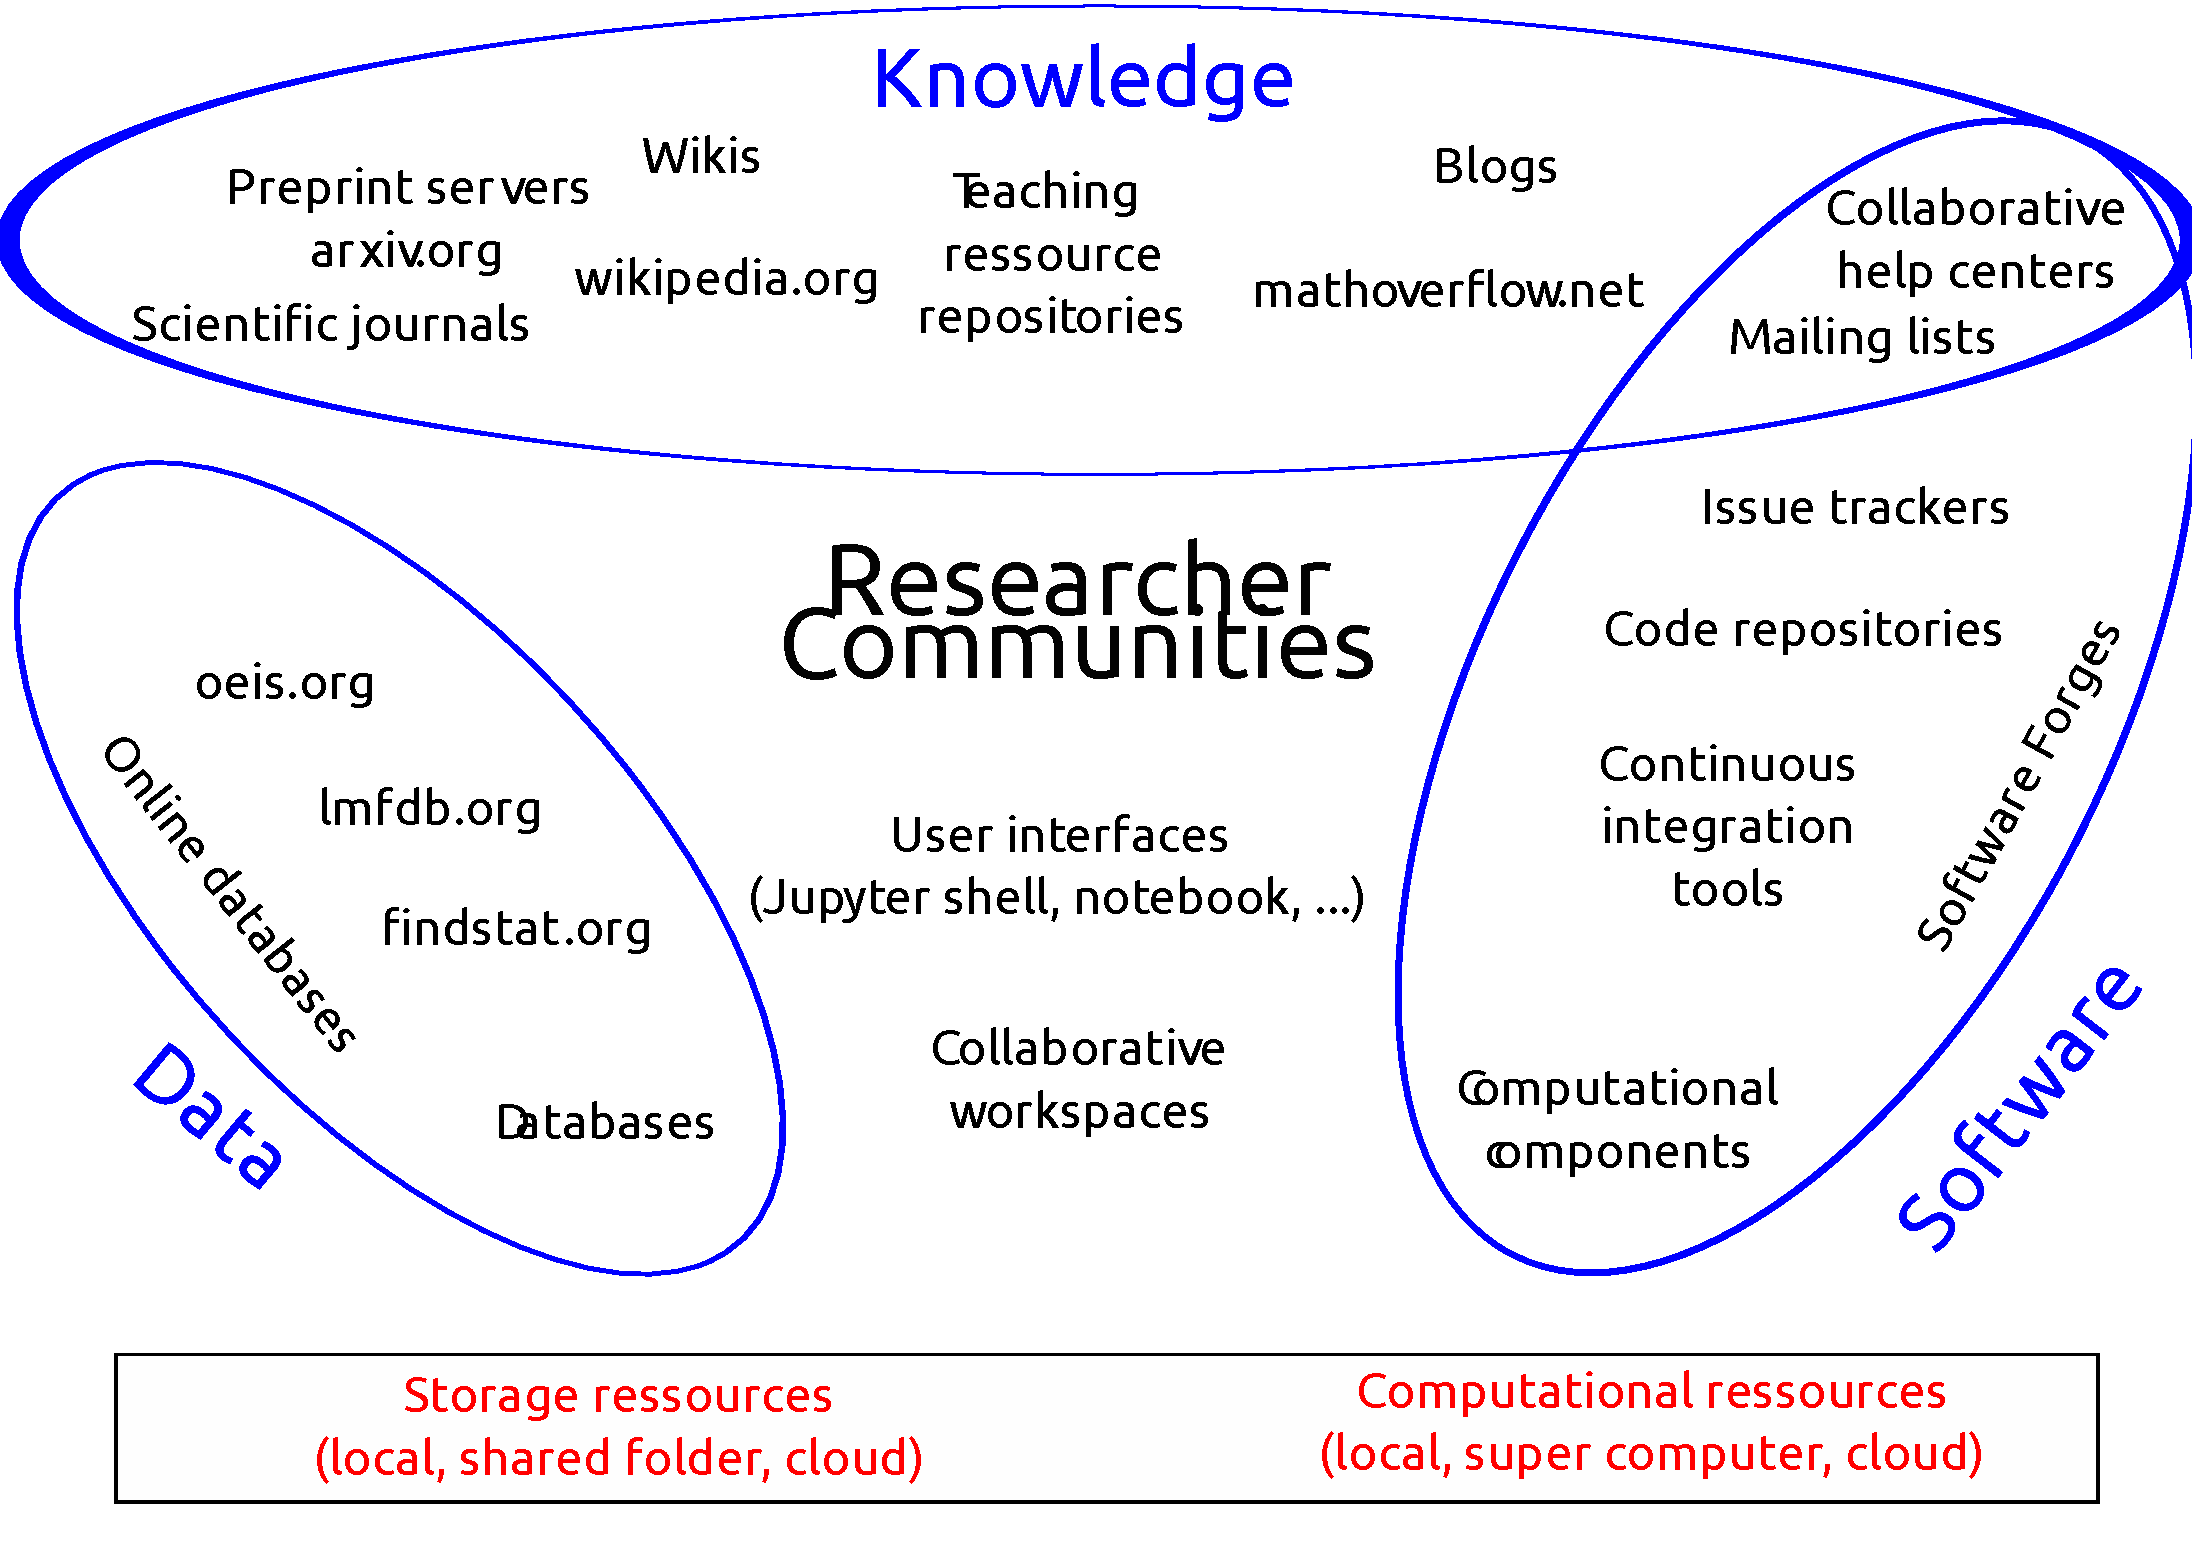
\includegraphics[width=\textwidth]{Pictures/TheBigPicture.pdf}}
  \caption{Virtual Research Environments for research in pure
    mathematics and applications.}
  \label{fig:thebigpicture}
\end{figure}

% \TODO{NT: the purpose of Figure~\ref{fig:thebigpicture} is to give a quick
%   sense of what Virtual Research Environments can be in our context,
%   and a ``big picture'' for the project. A graphic artist friend of
%   mine is going to help me improve it. I have collected here some material for her.\\\\
%   \textbf{\Large What we would like the ``big picture'' in
%     Figure~\ref{fig:thebigpicture} to highlight:}
%   \begin{description}
%   \item[This is a human centered project:] At the core: researchers and communities
%     thereof.
%   \item[The three types of information:]
%     Software, Knowledge, Data (currently in blue)\\
%     How they interact:
%     \begin{compactitem}
%     \item Knowledge help structure data and software (e.g. through ontologies)
%     \item Software produce data
%     \item Data is used by researchers to build knowledge
%     \end{compactitem}
%   \item[Physical resources:]
%     (currently in red)
%   \item[Virtual Research Environments]\ 
%     \begin{compactitem}
%     \item Researchers in Math have a long tradition of collaborating
%       on Software, Knowledge, and, up to some point, Data
%     \item For this they use a variety of collaborative tools which
%       form a loosely knit Virtual Research Environment.
%     \item \textbf{Aim 2}: make it easy for subcommunities of
%       researchers to set up custom collaborative work spaces / Virtual
%       Research Environments tailored to their needs, by combining:
%       \begin{compactitem}
%       \item Computational resources
%       \item Storage resources
%       \item Computational software components
%       \item Databases
%       \item User interfaces
%       \item Wikis-Knowledge bases (true for findstat, LMFDB): quicker
%         cycle for consolidation of information spread over
%         papers/brains
%       \end{compactitem}
%       Such VRE shall help them:
%       \begin{compactitem}
%       \item collaboratively develop software (e.g. specialized
%         libraries), data and knowledge (e.g. articles) for their
%         research projects.
%       \item contribute back this information to the larger community
%         whenever relevant.
%       \end{compactitem}
%     \end{compactitem}
%   \item[Processes:]\ \\
%     It would be interesting to depict the following processes. They
%     are indeed about collaboration and sharing (and quality control),
%     that is what \textbf{Aim 1} is to promote.
%     \begin{description}
%     \item[Software development]\ 
%       \begin{compactitem}
%       \item \emph{bug reports} and \emph{enhancement requests} emerge
%         from the community, typically through collaborative help
%         centers, and are posted on issue trackers.
%       \item \emph{Design discussions} occur on mailing lists and issue
%         trackers.
%       \item Researchers \emph{submit code} to the code repositories.
%       \item \emph{Quality control}: the code is reviewed and
%         tested by continuous integration tools.
%       \item Finally the code \emph{integrated} within computational
%         components, and used by the community.
%       \end{compactitem}
%       Researchers (as well as other users: teachers, engineers, ...)
%       interact at each step of the process.
%     \item[Scientific publication]\ 
%       \begin{compactitem}
%       \item researchers submit articles to journals and post them on
%         preprint servers;
%       \item the articles get reviewed by other researchers;
%       \item finally they are distributed back to the community
%       \end{compactitem}
%     \end{description}
%   \end{description}
%   %
%   Improvements to implement:
%   \begin{compactitem}
%   \item the findstat link does not work for me, kerning looks
%     extremely weird -- POD
%   \item LMFDB, OEIS, and findstat have a strong knowledge component as
%     well, with knowls and wikis, references, ...
%   \item arxiv is not far from a database of knowledge
%   \end{compactitem}
%   %
%   \textbf{\Large A collection of links that might give some idea of
%     the look and feel of our universe:}
%   \begin{description}
%   \item[Examples of (computational) components:]\ 
%     \begin{compactitem}
%     \item IPython: \url{http://ipython.org/}
%     \item GAP: \url{http://www.gap-system.org/}
%     \item Singular: \url{http://www.singular.uni-kl.de/}
%     \item Sage: \url{http://sagemath.org/}
%     \item \PariGP: \url{http://pari.math.u-bordeaux.fr/}
%     \item Linbox: \url{http://www.linalg.org/}
%     \end{compactitem}
%   \item[Examples of online collaborative tools]\ 
%     \begin{compactitem}
%     \item Issue tracker: \url{http://trac.sagemath.org/timeline/}
%     \item Code repository: \url{https://github.com/}
%     \item Collaborative help center: \url{http://ask.sagemath.org/}
%     \item Collaborative math site: \url{http://mathoverflow.net/}
%     \end{compactitem}
%   \item[Examples of online databases]\ 
%     \begin{compactitem}
%     \item Online databases: \url{http://oeis.org/?language=french}
%     \item LMFDB: \url{http://www.lmfdb.org/EllipticCurve/Q/14.a3}
%     \item Findstat: \url{http://www.findstat.org/}
%     \end{compactitem}
%   \item[Example of graphical material]\ 
%     \begin{compactitem}
%     \item \url{http://boxen.math.washington.edu/home/nthiery/main2014.pdf}
%     \end{compactitem}
%   \end{description}
% }
